% GNUPLOT: LaTeX picture with Postscript
\begingroup
  \makeatletter
  \providecommand\color[2][]{%
    \GenericError{(gnuplot) \space\space\space\@spaces}{%
      Package color not loaded in conjunction with
      terminal option `colourtext'%
    }{See the gnuplot documentation for explanation.%
    }{Either use 'blacktext' in gnuplot or load the package
      color.sty in LaTeX.}%
    \renewcommand\color[2][]{}%
  }%
  \providecommand\includegraphics[2][]{%
    \GenericError{(gnuplot) \space\space\space\@spaces}{%
      Package graphicx or graphics not loaded%
    }{See the gnuplot documentation for explanation.%
    }{The gnuplot epslatex terminal needs graphicx.sty or graphics.sty.}%
    \renewcommand\includegraphics[2][]{}%
  }%
  \providecommand\rotatebox[2]{#2}%
  \@ifundefined{ifGPcolor}{%
    \newif\ifGPcolor
    \GPcolortrue
  }{}%
  \@ifundefined{ifGPblacktext}{%
    \newif\ifGPblacktext
    \GPblacktexttrue
  }{}%
  % define a \g@addto@macro without @ in the name:
  \let\gplgaddtomacro\g@addto@macro
  % define empty templates for all commands taking text:
  \gdef\gplbacktext{}%
  \gdef\gplfronttext{}%
  \makeatother
  \ifGPblacktext
    % no textcolor at all
    \def\colorrgb#1{}%
    \def\colorgray#1{}%
  \else
    % gray or color?
    \ifGPcolor
      \def\colorrgb#1{\color[rgb]{#1}}%
      \def\colorgray#1{\color[gray]{#1}}%
      \expandafter\def\csname LTw\endcsname{\color{white}}%
      \expandafter\def\csname LTb\endcsname{\color{black}}%
      \expandafter\def\csname LTa\endcsname{\color{black}}%
      \expandafter\def\csname LT0\endcsname{\color[rgb]{1,0,0}}%
      \expandafter\def\csname LT1\endcsname{\color[rgb]{0,1,0}}%
      \expandafter\def\csname LT2\endcsname{\color[rgb]{0,0,1}}%
      \expandafter\def\csname LT3\endcsname{\color[rgb]{1,0,1}}%
      \expandafter\def\csname LT4\endcsname{\color[rgb]{0,1,1}}%
      \expandafter\def\csname LT5\endcsname{\color[rgb]{1,1,0}}%
      \expandafter\def\csname LT6\endcsname{\color[rgb]{0,0,0}}%
      \expandafter\def\csname LT7\endcsname{\color[rgb]{1,0.3,0}}%
      \expandafter\def\csname LT8\endcsname{\color[rgb]{0.5,0.5,0.5}}%
    \else
      % gray
      \def\colorrgb#1{\color{black}}%
      \def\colorgray#1{\color[gray]{#1}}%
      \expandafter\def\csname LTw\endcsname{\color{white}}%
      \expandafter\def\csname LTb\endcsname{\color{black}}%
      \expandafter\def\csname LTa\endcsname{\color{black}}%
      \expandafter\def\csname LT0\endcsname{\color{black}}%
      \expandafter\def\csname LT1\endcsname{\color{black}}%
      \expandafter\def\csname LT2\endcsname{\color{black}}%
      \expandafter\def\csname LT3\endcsname{\color{black}}%
      \expandafter\def\csname LT4\endcsname{\color{black}}%
      \expandafter\def\csname LT5\endcsname{\color{black}}%
      \expandafter\def\csname LT6\endcsname{\color{black}}%
      \expandafter\def\csname LT7\endcsname{\color{black}}%
      \expandafter\def\csname LT8\endcsname{\color{black}}%
    \fi
  \fi
  \setlength{\unitlength}{0.0500bp}%
  \begin{picture}(5040.00,2880.00)%
    \gplgaddtomacro\gplbacktext{%
      \colorrgb{0.61,0.61,0.61}%
      \put(546,1047){\makebox(0,0)[r]{\strut{}\footnotesize{1000}}}%
      \colorrgb{0.61,0.61,0.61}%
      \put(546,1240){\makebox(0,0)[r]{\strut{}\footnotesize{2000}}}%
      \colorrgb{0.61,0.61,0.61}%
      \put(546,1433){\makebox(0,0)[r]{\strut{}\footnotesize{3000}}}%
      \colorrgb{0.61,0.61,0.61}%
      \put(546,1626){\makebox(0,0)[r]{\strut{}\footnotesize{4000}}}%
      \colorrgb{0.61,0.61,0.61}%
      \put(546,1819){\makebox(0,0)[r]{\strut{}\footnotesize{5000}}}%
      \colorrgb{0.61,0.61,0.61}%
      \put(546,2011){\makebox(0,0)[r]{\strut{}\footnotesize{6000}}}%
      \colorrgb{0.61,0.61,0.61}%
      \put(546,2204){\makebox(0,0)[r]{\strut{}\footnotesize{7000}}}%
      \colorrgb{0.61,0.61,0.61}%
      \put(546,2397){\makebox(0,0)[r]{\strut{}\footnotesize{8000}}}%
      \colorrgb{0.61,0.61,0.61}%
      \put(546,2590){\makebox(0,0)[r]{\strut{}\footnotesize{9000}}}%
      \colorrgb{0.61,0.61,0.61}%
      \put(1121,888){\rotatebox{45}{\makebox(0,0)[r]{\strut{}\footnotesize{bgm}}}}%
      \colorrgb{0.61,0.61,0.61}%
      \put(1597,888){\rotatebox{45}{\makebox(0,0)[r]{\strut{}\footnotesize{stereovision0}}}}%
      \colorrgb{0.61,0.61,0.61}%
      \put(2074,888){\rotatebox{45}{\makebox(0,0)[r]{\strut{}\footnotesize{stereovision1}}}}%
      \colorrgb{0.61,0.61,0.61}%
      \put(2550,888){\rotatebox{45}{\makebox(0,0)[r]{\strut{}\footnotesize{LU8PEEng}}}}%
      \colorrgb{0.61,0.61,0.61}%
      \put(3026,888){\rotatebox{45}{\makebox(0,0)[r]{\strut{}\footnotesize{mkDelayWorker32B}}}}%
      \colorrgb{0.61,0.61,0.61}%
      \put(3502,888){\rotatebox{45}{\makebox(0,0)[r]{\strut{}\footnotesize{stereovision2}}}}%
      \colorrgb{0.61,0.61,0.61}%
      \put(3979,888){\rotatebox{45}{\makebox(0,0)[r]{\strut{}\footnotesize{mcml}}}}%
      \colorrgb{0.61,0.61,0.61}%
      \put(4455,888){\rotatebox{45}{\makebox(0,0)[r]{\strut{}\footnotesize{LU32PEEng}}}}%
      \csname LTb\endcsname%
      \put(48,1818){\rotatebox{-270}{\makebox(0,0){\strut{}\footnotesize{\textbf{Blocks in Clustered Netlist}}}}}%
      \put(2788,42){\makebox(0,0){\strut{}\footnotesize{\textbf{Circuit}}}}%
    }%
    \gplgaddtomacro\gplfronttext{%
      \csname LTb\endcsname%
      \put(924,2739){\makebox(0,0)[l]{\strut{}\footnotesize{No Packing Constraints}}}%
      \csname LTb\endcsname%
      \put(2931,2739){\makebox(0,0)[l]{\strut{}\footnotesize{Packing Constraints}}}%
    }%
    \gplbacktext
    \put(0,0){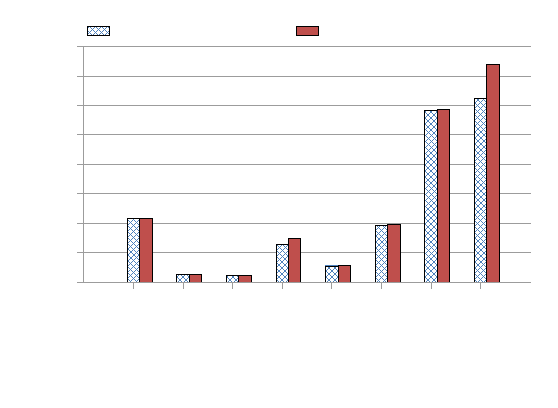
\includegraphics{packing_bloat}}%
    \gplfronttext
  \end{picture}%
\endgroup
